%!TEX program = xelatex
\documentclass[cn,blue,normal,11pt]{elegantnote}
\usepackage{url}
\usepackage{multirow}
\usepackage{listings}
% 在LaTex中添加代码
\usepackage{color}
\usepackage{tabu}
% \definecolor{codegreen}{rgb}{0,0.6,0}
% \definecolor{codegray}{rgb}{0.5,0.5,0.5}
% \definecolor{codepurple}{rgb}{0.58,0,0.82}
% \definecolor{backcolour}{rgb}{0.95,0.95,0.92}



\title{ElegantNote:一个优美的 \LaTeX{} 笔记模板}

\author{\href{https://ddswhu.me/}{邓东升}}
\institute{\href{https://elegantlatex.org/}{Elegant\LaTeX{} Program}}
\version{2.20}
\date{\today}


\begin{document}
% \maketitle
% % logo
% \centerline{
\includegraphics[width=0.25\textwidth]{logo.pdf}}

% \setlist[itemize]{label=$\circ$}
\textbf{版本}

\begin{table}[htbp]
    \centering
    \begin{tabular}{|c|c|c|c|c|}
        \hline
        \multirow{4}{*}{\textbf{更新记录}} & \multicolumn{2}{c|}{文档名} & \multicolumn{2}{c|}{实验指导书\_lab3} \\
        % \hline
        \cline{2-5} & \multicolumn{2}{c|}{版本号} & \multicolumn{2}{c|}{0.3} \\
        \cline{2-5} & \multicolumn{2}{c|}{创建人} & \multicolumn{2}{c|}{计算机组成原理教学组} \\
        \cline{2-5} & \multicolumn{2}{c|}{创建日期} & \multicolumn{2}{c|}{2017/11/3} \\
        \hline
        \multicolumn{5}{|l|}{\textbf{更新历史}} \\
        \hline
        \textbf{序号} & \textbf{更新日期} & \textbf{更新人} & \textbf{版本号} & \textbf{更新内容} \\
        \hline 
        1 & 2017/11/5 & 吕昱峰 & 0.1 & 初版,单周期CPU取指译码实验\\
        \hline
        2 & 2018/11/5 & 吕昱峰 & 0.2 & 重新组织指导书内容。\\
        \hline
        3 & 2019/11/21 & 吕昱峰 & 0.3 & 完善设计连线的描述内容,阅读更加易于理解。\\
        \hline
         & & & & \\
        \hline
    \end{tabular}
    % \caption{Caption}
    \label{tab:guide_book_version}
\end{table}


文档错误反馈:\url{lvyufeng@cqu.edu.cn}

\newpage

\section{实验三 \quad 简易单周期CPU实验}
MIPS架构CPU的传统流程可分为\textit{取指、译码、执行、访存、回写}(Instruction Fetch, Decode, Execution, Memory Request, Write Back),五阶段。

实验一完成了ALU设计并掌握了存储器IP的使用;实验二实现了单周期CPU的取指、译码阶段,完成了PC、控制器的设计。在实验一与实验二的基础上,单周期CPU的设计的各模块已经具备,再引入数字逻辑课程中所实现的多路选择器、加法器等门级组件,通过对原理图的理解,分析单条(单类型)指令在数据通路中的执行路径,依次连接对应端口,即可完成单周期CPU。

在进行本次实验前,你需要具备以下基础能力:
\begin{enumerate}
    \item 熟悉Vivado的仿真功能(行为仿真)
    \item 理解数据通路、控制器的信号
\end{enumerate}

\subsection{实验目的}
\begin{enumerate}
    \item 掌握不同类型指令在数据通路中的执行路径。
    \item 掌握Vivado仿真方式。
\end{enumerate}
\subsection{实验设备}
\begin{enumerate}
    \item 计算机1台(尽可能达到8G及以上内存);
    \item Xilinx Vivado开发套件(2019.1版本)。
\end{enumerate}
\textcolor{red}{注:本次实验为CPU软核实验,不涉及开发板外围设备,故不需要开发板
}
\subsection{实验任务}
\subsubsection{实验要求}
阅读实验原理实现以下模块:
\begin{enumerate}[(1)]
    \item Datapath,其中主要包含alu(实验一已完成),PC(实验二已完成),adder、mux2、signext、sl2(其中adder、mux2数字逻辑课程已实现,signext、sl2参见实验原理),
    \item Controller(实验二已完成),其中包含两部分,分别为main\_decoder,alu\_decoder。
    \item 指令存储器inst\_mem(Single Port Ram),数据存储器data\_mem(Single Port Ram);使用Block Memory Generator IP构造指令,注意考虑PC地址位数统一。(参考实验二)
    \item 参照实验原理,将上述模块依指令执行顺序连接。实验给出top文件,需兼容top文件端口设定。
    \item 实验给出仿真程序,最终以仿真输出结果判断是否成功实现要求指令。
\end{enumerate}

\subsubsection{实验步骤}
\begin{enumerate}
    \item 从实验一中,导入alu模块;
    \item 从实验二中导入PC、Controller模块;
    \item 从数字逻辑实验中导入多路选择器、加法器模块;
    \item 使用Block Memory,其中inst\_mem导入coe文件;
    \item 参考实验原理,连接各模块;
    \item 导入顶层文件及仿真文件,运行仿真; 
\end{enumerate}

\subsection{实验环境}
\begin{table}[htbp]
    \centering
    \begin{tabular}{|l|l|}
        \hline
        |--top.v& 设计顶层文件,已提供。 \\
        |----mips.v & MIPS软核顶层文件,将Controller与Datapath连接,已提供 \\
        % \textcolor{red}{|----pc.v} &\textcolor{red}{D触发器结构。输入为下一条指令地址,输出为当前指令地址。}  \\
        % |----ram.ip&RAM IP,通过Block memory generator进行实例化。  \\
        \textcolor{blue}{|------controller.v} &\textcolor{blue}{ 控制器模块,本次实验重点。} \\
        \textcolor{blue}{|--------maindec.v} & \textcolor{blue}{Main decoder模块,负责译码得到各个组件的控制信号。} \\
        \textcolor{blue}{|--------aludec.v} & \textcolor{blue}{ALU Decoder模块,负责译码得到ALU控制信号。}\\
        \textcolor{red}{|------datapath.v}& \textcolor{red}{数据通路模块,自行实现} \\
        \textcolor{blue}{|--------pc.v} & \textcolor{blue}{PC模块,使用实验二代码} \\
        \textcolor{blue}{|--------alu.v} & \textcolor{blue}{ALU模块,使用实验一代码} \\
        \textcolor{green}{|--------sl2.v} & \textcolor{green}{移位模块,参考《其他组件实现.pdf》} \\
        \textcolor{green}{|--------signext.v} & \textcolor{green}{有符号扩展模块,参考《其他组件实现.pdf》} \\
        \textcolor{red}{|--------mux2.v} & \textcolor{red}{二选一选择器,自行实现} \\
        \textcolor{black}{|--------regfile.v} & \textcolor{black}{寄存器堆,已提供} \\
        \textcolor{black}{|--------adder.v} & \textcolor{black}{加法器,已提供} \\
        \textit{|----inst\_ram.ip} & \textit{RAM IP,通过Block memory generator进行实例化}\\
        \textit{|----data\_ram.ip} & \textit{RAM IP,通过Block memory generator进行实例化}\\
        \hline
    \end{tabular}
    \caption{实验文件树}
    \label{tab:file_tree}
\end{table}

\newpage

\section{流水线}
\subsection{流水线原理}
\subsubsection{什么是流水线}
流水线设计就是将组合逻辑系统地分割,并在各个部分(分级)之间插入寄存器,并暂存中间数据的方法。目的是将一个大操作分解成若干的小操作,每一步小操作的时间较小,所以能提高频率,各小操作能并行执行,所以能提高数据吞吐率(提高处理速度)。

\subsubsection{什么时候用流水线设计}
使用流水线一般是时序比较紧张,对电路工作频率较高的时候。典型情况如下:
\begin{enumerate}
    \item 功能模块之间的流水线,用乒乓 buffer 来交互数据。代价是增加了 memory 的数量,但是和获得的巨大性能提升相比,可以忽略不计。
    \item I/O 瓶颈,比如某个运算需要输入 8 个数据,而 memroy 只能同时提供 2个数据,如果通过适当划分运算步骤,使用流水线反而会减少面积。
    \item 片内 sram的读操作,因为sram的读操作本身就是两极流水线,除非下一步操作依赖读结果,否则使用流水线是自然而然的事情。
    \item 组合逻辑太长,比如(a+b)*c,那么在加法和乘法之间插入寄存器是比较稳妥的做法。
\end{enumerate}

\subsubsection{使用流水线的优缺点}

\textbf{优点}:流水线缩短了在一个时钟周期内给的那个信号必须通过的通路长度,增加了数据吞吐量,从而可以提高时钟频率,但也导致了数据的延时。
% 举例如下:

% 一个 2 级组合逻辑,假定每级延迟相同为 Tpd,
% \begin{enumerate}
%     \item 无流水线的总延迟就是2Tpd,可以在一个时钟周期完成,但是时钟周期受限制在 2Tpd;
%     \item 流水线:
%     每一级加入寄存器(延迟为 Tco)后,单级的延迟为 Tpd+Tco,每级消耗一个时钟周期,流水线需要 2 个时钟周期
%     来获得第一个计算结果,称 为首次延迟,它要 2*( Tpd+Tco),但是执行重复操作时,只要一个时钟周期来获得最后的
%     计算结果,称为吞吐延迟( Tpd+Tco)。可见只要 Tco 小于 Tpd,流水线就可以提高速度。 特别需要说明的是,流水线
%     并不减小单次操作的时间,减小的是整个数据的操作时间,请大家认真体会。
% \end{enumerate}

\textbf{缺点}: 功耗增加,面积增加,硬件复杂度增加,特别对于复杂逻辑如 CPU 的流水线而言,流水越深,发生需要暂停流水线或刷新流水线的情况时,时间损失越大。

所以使用流水线并非有利无害,设计时需权衡考虑。


\subsection{流水线基础示例}
首先要说明的一点是,流水线电路纯粹就是一个数字电路的概念,不要一谈到流水线就仅仅认为是处理器中 的流水线。

我们先来看一个完全不会被阻塞的 3 级流水线电路怎么写。
\begin{lstlisting}[language=Verilog,label=lst:3_stage_pipeline,caption=无阻塞3级流水线实现,numbers=left,xleftmargin=5em,xrightmargin=5em, aboveskip=2em]
module non_stall_pipeline #
(
    parameter WIDTH = 100
)
(
    input              clk,
    input  [WIDTH-1:0] datain,
    output [WIDTH-1:0] dataout
);

reg [WIDTH-1:0] pipe1_data;
reg [WIDTH-1:0] pipe2_data;
reg [WIDTH-1:0] pipe3_data;

always @(posedge clk) begin
    pipe1_data <= datain;
end

always @(posedge clk) begin
    pipe2_data <= pipe1_data;
end

always @(posedge clk) begin
    pipe3_data <= pipe2_data;
end

assign dataout = pipe3_data;

endmodule
\end{lstlisting}

但是实际电路设计中,并不总是上面这种无阻塞的流水线。下面给出一个具有阻塞功能的流水线代码。
\begin{lstlisting}[language=Verilog,label=lst:3_stage_pipeline_stall_flush,caption=有阻塞3级流水线实现,numbers=left,xleftmargin=5em,xrightmargin=5em, aboveskip=2em]
module stallable_pipeline #
(
parameter WIDTH = 100
)
(
input              clk,
input              rst,
input              validin,
input  [WIDTH-1:0] datain,
input              out_allow,
output             validout,
output [WIDTH-1:0] dataout
);

reg             pipe1_valid;
reg [WIDTH-1:0] pipe1_data;
reg             pipe2_valid;
reg [WIDTH-1:0] pipe2_data;
reg             pipe3_valid;
reg [WIDTH-1:0] pipe3_data;

// pipeline stage1
wire            pipe1_allowin;
wire            pipe1_ready_go;
wire            pipe1_to_pipe2_valid;

assign pipe1_ready_go = ……
assign pipe1_allowin = !pipe1_valid || pipe1_ready_go && pipe2_allowin;
assign pipe1_to_pipe2_valid = pipe1_valid && pipe1_ready_go;

always @(posedge clk) begin
    if (rst) begin
        pipe1_valid <= 1’b0;
    end
    else if (pipe1_allowin) begin
        pipe1_valid <= validin;
    end
    if (validin && pipe1_allowin) begin
        pipe1_data <= datain;
    end
end

// pipeline stage2
wire            pipe2_allowin;
wire            pipe2_ready_go;
wire            pipe2_to_pipe3_valid;

assign pipe2_ready_go = ……
assign pipe2_allowin = !pipe2_valid || pipe2_ready_go && pipe3_allowin;
assign pipe2_to_pipe3_valid = pipe2_valid && pipe2_ready_go;

always @(posedge clk) begin
    if (rst) begin
        pipe2_valid <= 1’b0;
    end
    else if (pipe2_allowin) begin
        pipe2_valid <= pipe1_to_pipe2_valid;
    end
    if (pipe1_to_pipe2_valid && pipe2_allowin) begin
        pipe2_data <= pipe1_data;
    end
end

// pipeline stage3
wire            pipe3_allowin;
wire            pipe3_ready_go;

assign pipe3_ready_go = ……
assign pipe3_allowin = !pipe3_valid || pipe3_ready_go && out_allow;

always @(posedge clk) begin
    if (rst) begin
        pipe3_valid <= 1’b0;
    end
    else if (pipe3_allowin) begin
        pipe3_valid <= pipe2_to_pipe3_valid;
    end
    if (pipe2_to_pipe3_valid && pipe3_allowin) begin
        pipe3_data <= pipe2_data;
    end
end

assign validout = pipe3_valid && pipe3_ready_go;
assign dataout  = pipe3_data;

endmodule
\end{lstlisting}

上述代码表述中pipe\textbf{X}\_valid为1表示第X级流水级上当前存有有效的数据,为0表示第X级是空的。因为控制位的好处是,清空流水线的时候不用刷各级流水线data域的值,可以节约逻辑资源,但是需要注意的是根据流水 级的data域信息产生控制信号时,有时候不要忘记“与上”这一级的 valid 信号。

pipe\textbf{X}\_allowin为1表示第X级可以接收前一级流水送来的数据。

上面流水线的 RTL 写法对于流水级的关键控制信号采用了链式写法。这样写的好处是,如果发生流水级功能调整时,譬如将一级再切分为两级,或者将某一级的停顿周期数改变了,都只需要修改局部,不会涉及全局性的 调整。有的同学可能会觉得我这种写法很麻烦,觉得自己写出来的简单一些。请你们针对具体情况分析,是否对于你所涉及的流水线,上面给出的代码中,某些pipeX\_allowin和pipeX\_ready\_go可以恒置为1,将其代入上面的表达式中,并将级联的控制信号完全展开,就形成了你们的那种简单版本。这里给出这样的一个流水线电路的“模板”式写法,主要是因为它易于理解不易出错,当同学们在自己进行流水线设计时如果因为流水级控制信号 搞得很糊涂时,可以回过头来看看此处给出的例子。

再额外说一点,上面的写法是把流水线的 control logic 和 data path 写到了一个模块内部。你也可以把两者分在不同的模块中。国外的教科书上在描述流水线 CPU 时,通常会在流水线之外画一个叫做 pipeline control logic 的椭圆形框,从这个框引出控制信号去往各级流水所在触发器的使能端。这就是把 control logic 和 data path 分离的写法。 我们在上面给出的例子,pipeX\_data 就是 data path主体。
 
\subsection{8bit全加器示例}
\subsubsection{非流水线方式}
\begin{lstlisting}[language=Verilog,label=lst:no_stage,caption=8bit全加器非流水线实现,numbers=left,xleftmargin=5em,xrightmargin=5em, aboveskip=2em]
module adder_8bits(
    a, 
    b, 
    c
);
input  [7:0] a;
input  [7:0] b;
output [8:0] c;

assign c[8:0] = {1'd0, a} + {1'd0, b};
endmodule
\end{lstlisting}
\subsubsection{2级流水线}
\begin{lstlisting}[language=Verilog,label=lst:2_stage_pipeline,caption=8bit全加器2级流水线实现,numbers=left,xleftmargin=5em,xrightmargin=5em, aboveskip=2em]
module adder_4bits_2steps(cin_a, cin_b, cin, clk, cout, sum);
input [7:0]     cin_a;
input [7:0]     cin_b;
input           cin;
input           clk;
output          cout;
output [7:0]    sum;
	 
reg         cout;
reg         cout_temp;
reg [7:0]   sum;
reg [3:0]   sum_temp;
	 
always @(posedge clk) begin
    {cout_temp,sum_temp} <= cin_a[3:0] + cin_b[3:0] + cin;
end
	 
always @(posedge clk) begin
    {cout,sum} <= {{1'b0,cin_a[7:4]} + {1'b0,cin_b[7:4]} + cout_temp, sum_temp};
end
endmodule
\end{lstlisting}
\subsubsection{4级流水线}
\begin{lstlisting}[language=Verilog,label=lst:4_stage_pipeline,caption=8bit全加器4级流水线实现,numbers=left,xleftmargin=5em,xrightmargin=5em, aboveskip=2em]
module adder_8bits_4steps(cin_a, cin_b, c_in, clk, c_out, sum_out);
input [7:0]     cin_a;
input [7:0]     cin_b;
input           c_in;
input           clk;
output          c_out;
output [7:0]    sum_out;
	 
reg c_out;
reg c_out_t1, c_out_t2, c_out_t3;
	 
reg [7:0] sum_out;
reg [1:0] sum_out_t1;
reg [3:0] sum_out_t2;
reg [5:0] sum_out_t3;
	 
always @(posedge clk) begin
    {c_out_t1, sum_out_t1} <= {1'b0, cin_a[1:0]} + {1'b0, cin_b[1:0]} + c_in;
end
	 
always @(posedge clk) begin
    {c_out_t2, sum_out_t2} <= {{1'b0, cin_a[3:2]} + {1'b0, cin_b[3:2]} + c_out_t1, sum_out_t1};
end
	 
always @(posedge clk) begin
    {c_out_t3, sum_out_t3} <= {{1'b0, cin_a[5:4]} + {1'b0, cin_b[5:4]} + c_out_t2, sum_out_t2};
end
	 
always @(posedge clk) begin
    {c_out, sum_out} <= {{1'b0, cin_a[7:6]} + {1'b0, cin_b[7:6]} + c_out_t3, sum_out_t3};
end

endmodule
\end{lstlisting}


\newpage

\section{Verilog不同实现方式}
验证实验给出两种不同的组合逻辑实现方式:

\begin{lstlisting}[language=Verilog,label=lst:assign,caption=assign实现组合逻辑,numbers=left,xleftmargin=5em,xrightmargin=5em, aboveskip=2em]
module calculate(
    input wire [7:0] num1,
    input wire [2:0] op,
    output [31:0] result
    );
    wire [31:0] num2;
    wire [31:0] Sign_extend;
    
    assign num2 = 32'h00000001;
    assign Sign_extend={{24{1'b0}},num1[7:0]};
    assign result = (op == 3'b000)? Sign_extend + num2:
                    (op == 3'b001)? Sign_extend - num2:
                    (op == 3'b010)? Sign_extend & num2:
                    (op == 3'b011)? Sign_extend | num2:
                    (op == 3'b100)? ~Sign_extend: 32'h00000000;
endmodule
\end{lstlisting}


\begin{lstlisting}[language = Verilog,label=lst:always,caption=always实现组合逻辑,numbers=left,xleftmargin=5em,xrightmargin=5em, aboveskip=2em]
module calculate(
    input wire [7:0] num1,
    input wire [2:0] op,
    output reg [31:0] result
    );
    reg [31:0] num2;
    reg[31:0] Sign_extend;
    always @(op) begin
       num2 = 32'h00000001;
       Sign_extend={24'h000000,num1[7:0]};
            case(op)
                3'b000:result = Sign_extend + num2;
                3'b001:result = Sign_extend - num2; 
                3'b010:result = Sign_extend &  num2;
                3'b011:result = Sign_extend |  num2;
                3'b100:result = ~Sign_extend  ;          
                default:result = 32'h00000000;
            endcase
        end
endmodule
\end{lstlisting}

二者区别对比如下:

\begin{table}[htbp]
    \centering
    \begin{tabular}{c|c|c}
          \hline
          & assign & always  \\
          \hline
          result    & wire & reg \\
          num2      & wire  & reg \\
          sign\_extend & wire &  reg\\
          \hline
    \end{tabular}
    \caption{assign \& always 信号对比}
    \label{tab:sig_compare}
\end{table}
Always即可实现组合逻辑,也可实现时序逻辑:
\begin{enumerate}[(1)]
    \item always @(a or b or c)或always@(*)形式的,即不带时钟边沿的,综合出来还是组合逻辑;
    \item always @(posedge clk)形式的,即带有边沿的,综合出来一般是时序逻辑,会包含触发器(Flip-Flop)
\end{enumerate}

观察Listing~\ref{lst:always}中always的触发信号op,可以得知其为组合逻辑。在这里,给出两种方式在FPGA资源及编程难度上的对比。


\begin{table}[htbp]
    \centering
    \begin{tabular}{c|p{5cm}|p{5cm}}
         \hline
          & assign & always \\
         \hline
         资源占用  &  使用wire变量,综合得到的组合逻辑全部由导线构成,不占用FPGA资源 & 由于内部赋值与输出都需要使用reg变量,同为组合逻辑,需占用一定资源 \\
         \hline
         编程及理解难度 & 面向信号进行状态描述,一般需要考虑单个信号在所有状态下的可能性,需要完全理解后进行编程。
        
        阅读者理解难度大。
        & 面向实验需求描述,always模块内书写方式与高级语言相仿,可以按照实验要求逐一列举。

        阅读者理解较容易。
        \\
         \hline
    \end{tabular}
    \caption{assign \& always 设计对比}
    \label{tab:design_compare}
\end{table}

\textcolor{red}{\textbf{注意:}}\textbf{Imagination及龙芯高校开源计划代码均采取assign方式,实验推荐使用assign方式实现组合逻辑。设计实验中新增内容使用assign方式增加输出信号更为简单。}

\newpage

\appendix
\section{Nexys4 DDR开发板基本信息}

\begin{figure}[htbp]
    \centering
    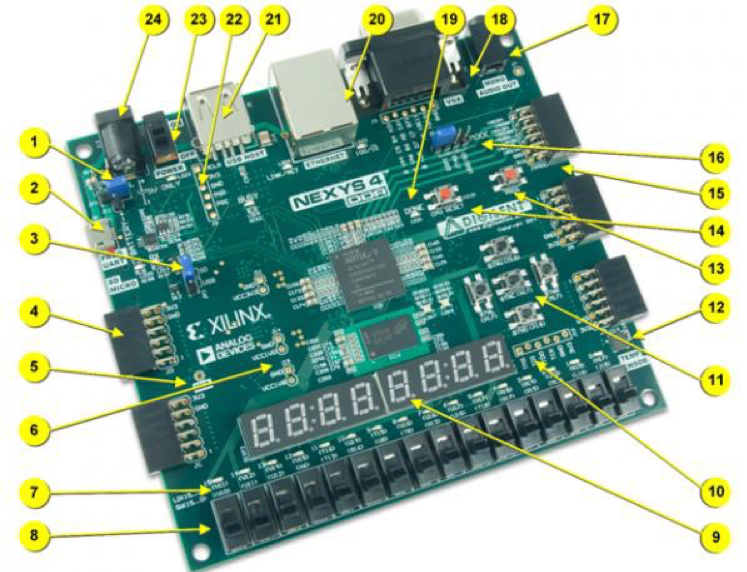
\includegraphics[width = 0.75\textwidth]{image/appendix/appendix_a_0.png}
    \caption{Nexys4 DDR示意图}
    \label{fig:appendix_a_0}
\end{figure}

\begin{table}[htbp]
    \centering
    \begin{tabular}{cc|cc}
         1& 选择供电跳线 &   13 & FPGA配置复位按键 \\
         2& UART/ JTAG 共用 USB 接口 &   14 & CPU 复位按键 (用于软核)\\
         3& 外部配置跳线柱(SD / USB) &   15& 模拟信号 Pmod 端口(XADC)\\
         4& Pmod 端口 &   16&编程模式跳线柱 \\
         5& 扩音器 &   17&音频连接口 \\
         6& 电源测试点 &   18& VGA 连接口\\
         7& 16 个 LED &   19& FPGA 编程完成 LED\\
         8& 16 个拨键开关&   20&以太网连接口 \\
         9& 8 位 7 段数码管&   21&USB 连接口 \\
         10& 可选用于外部接线的 JTAG 端口&  22&(工业用) PIC24 编程端口 \\
         11& 5 个按键开关 &  23& 电源开关\\
         12& 板载温度传感器 &  24&电源接口 \\
        %  & & & \\
    \end{tabular}
    \caption{Nexys4 DDR 功能表}
    \label{tab:my_label}
\end{table}

\newpage
\section{Nexys4 DDR引脚说明}
\textbf{100MHz时钟  E3}

按键、拨码管、LED、七段数码管、Reset:
\begin{figure}[htbp]
    \centering
    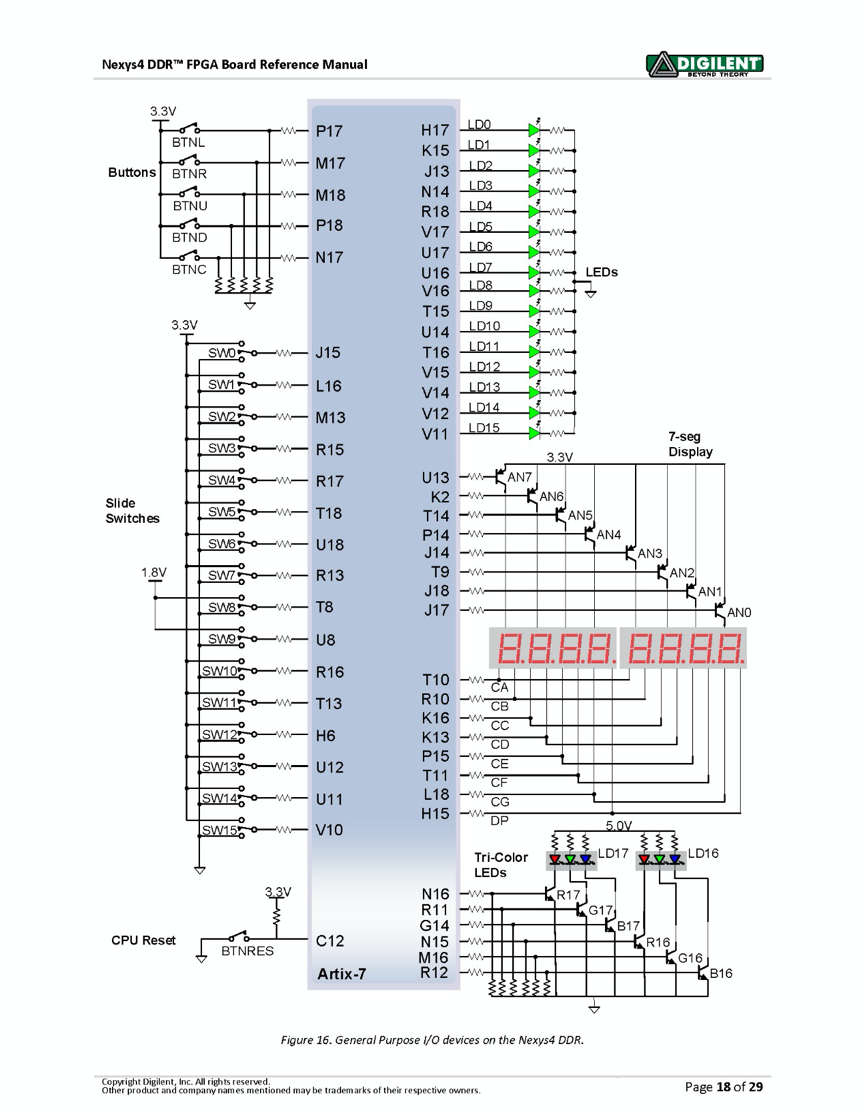
\includegraphics[width  = 0.9\textwidth]{image/appendix/appendix_b_0.png}
    \caption{Nexys4 DDR 管脚图}
    \label{fig:my_label}
\end{figure}

\newpage
\section{七段数码管的使用}
Nexys4 DDR实验板上有两个4位带小数点的七段数码管,图~\ref{fig:appendix_c_0}显示了它们与主芯片的连接方式。其中A7~A0是数码管8个位的使能信号,而CA~CG/DP则对应各个位上七个段以及小数点的触发信号。需要注意的是,使能信号和触发信号都是低电平触发的。

\begin{figure}[htbp]
    \centering
    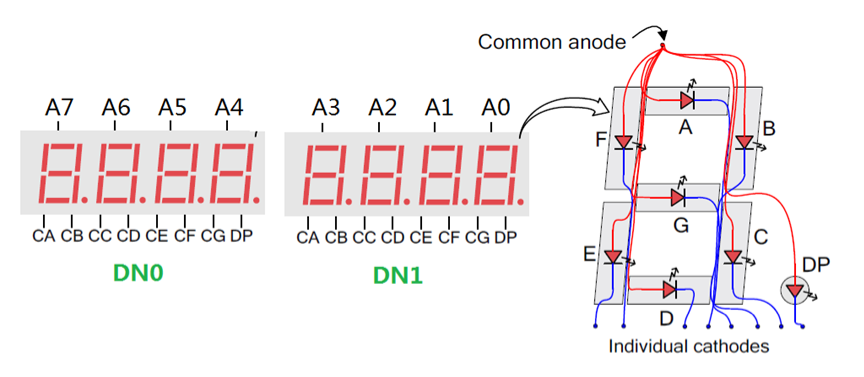
\includegraphics[width = \textwidth]{image/appendix/appendix_c_0.png}
    \caption{七段数码管示意图}
    \label{fig:appendix_c_0}
\end{figure}

图~\ref{fig:appendix_c_0}以数码管中最右侧的A0数码管为例说明了Nexys4 DDR板卡上的7-段数码管的连接方式。8个位中的各个相应的段及小数点分别连接到一组低电平触发的引脚上,他们被称为CA、CB、CC、…、CG、DP,其中,CA接到这8个数码管中每一个数码管A段的负极,CB接到这8个数码管中每一个数码管B段的负极,以此类推。

此外,每一个数码管都有一个使能信号A[7:0]。A[7:0]通过一个反相器接到对应数码管的每一个段的正极上。比如说,只有到A[0]为0的时候,最右侧数码管的显示才会受到CA…CG这几个信号的驱动。

图~\ref{fig:appendix_c_1}中列出了数码管显示0到F时点亮的段。比如说在显示数字0的时候,除了中间的G段外其他的段都被点亮了。而数字1只点亮了B段和C段。

\begin{figure}[htbp]
    \centering
    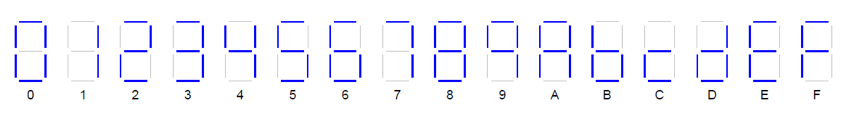
\includegraphics[width = \textwidth]{image/appendix/appendix_c_1.png}
    \caption{0-F点亮示意图}
    \label{fig:appendix_c_1}
\end{figure}

要想让每个数码管显示不同的数字,使能信号(A[7:0])和段信号(CA…CG)必须依次地被持续驱动,数码管之间的刷新速度应该足够快这样就看不出来数码管之间在闪烁。举个例子,如果想在数码管0上显示数字3而数码管1上显示数字9,可以先把CA…CG设置为显示数字3,并拉低A[1]信号,然后再把CA…CG设置为显示数字9并拉高A[1]拉低A[2]。刷新频率可以设置为2ms刷新一次,这样人眼就看不出闪烁了。
% \newpage

% \section{实验三 \quad 简易单周期CPU实验}
MIPS架构CPU的传统流程可分为\textit{取指、译码、执行、访存、回写}(Instruction Fetch, Decode, Execution, Memory Request, Write Back),五阶段。

实验一完成了ALU设计并掌握了存储器IP的使用;实验二实现了单周期CPU的取指、译码阶段,完成了PC、控制器的设计。在实验一与实验二的基础上,单周期CPU的设计的各模块已经具备,再引入数字逻辑课程中所实现的多路选择器、加法器等门级组件,通过对原理图的理解,分析单条(单类型)指令在数据通路中的执行路径,依次连接对应端口,即可完成单周期CPU。

在进行本次实验前,你需要具备以下基础能力:
\begin{enumerate}
    \item 熟悉Vivado的仿真功能(行为仿真)
    \item 理解数据通路、控制器的信号
\end{enumerate}

\subsection{实验目的}
\begin{enumerate}
    \item 掌握不同类型指令在数据通路中的执行路径。
    \item 掌握Vivado仿真方式。
\end{enumerate}
\subsection{实验设备}
\begin{enumerate}
    \item 计算机1台(尽可能达到8G及以上内存);
    \item Xilinx Vivado开发套件(2019.1版本)。
\end{enumerate}
\textcolor{red}{注:本次实验为CPU软核实验,不涉及开发板外围设备,故不需要开发板
}
\subsection{实验任务}
\subsubsection{实验要求}
阅读实验原理实现以下模块:
\begin{enumerate}[(1)]
    \item Datapath,其中主要包含alu(实验一已完成),PC(实验二已完成),adder、mux2、signext、sl2(其中adder、mux2数字逻辑课程已实现,signext、sl2参见实验原理),
    \item Controller(实验二已完成),其中包含两部分,分别为main\_decoder,alu\_decoder。
    \item 指令存储器inst\_mem(Single Port Ram),数据存储器data\_mem(Single Port Ram);使用Block Memory Generator IP构造指令,注意考虑PC地址位数统一。(参考实验二)
    \item 参照实验原理,将上述模块依指令执行顺序连接。实验给出top文件,需兼容top文件端口设定。
    \item 实验给出仿真程序,最终以仿真输出结果判断是否成功实现要求指令。
\end{enumerate}

\subsubsection{实验步骤}
\begin{enumerate}
    \item 从实验一中,导入alu模块;
    \item 从实验二中导入PC、Controller模块;
    \item 从数字逻辑实验中导入多路选择器、加法器模块;
    \item 使用Block Memory,其中inst\_mem导入coe文件;
    \item 参考实验原理,连接各模块;
    \item 导入顶层文件及仿真文件,运行仿真; 
\end{enumerate}

\subsection{实验环境}
\begin{table}[htbp]
    \centering
    \begin{tabular}{|l|l|}
        \hline
        |--top.v& 设计顶层文件,已提供。 \\
        |----mips.v & MIPS软核顶层文件,将Controller与Datapath连接,已提供 \\
        % \textcolor{red}{|----pc.v} &\textcolor{red}{D触发器结构。输入为下一条指令地址,输出为当前指令地址。}  \\
        % |----ram.ip&RAM IP,通过Block memory generator进行实例化。  \\
        \textcolor{blue}{|------controller.v} &\textcolor{blue}{ 控制器模块,本次实验重点。} \\
        \textcolor{blue}{|--------maindec.v} & \textcolor{blue}{Main decoder模块,负责译码得到各个组件的控制信号。} \\
        \textcolor{blue}{|--------aludec.v} & \textcolor{blue}{ALU Decoder模块,负责译码得到ALU控制信号。}\\
        \textcolor{red}{|------datapath.v}& \textcolor{red}{数据通路模块,自行实现} \\
        \textcolor{blue}{|--------pc.v} & \textcolor{blue}{PC模块,使用实验二代码} \\
        \textcolor{blue}{|--------alu.v} & \textcolor{blue}{ALU模块,使用实验一代码} \\
        \textcolor{green}{|--------sl2.v} & \textcolor{green}{移位模块,参考《其他组件实现.pdf》} \\
        \textcolor{green}{|--------signext.v} & \textcolor{green}{有符号扩展模块,参考《其他组件实现.pdf》} \\
        \textcolor{red}{|--------mux2.v} & \textcolor{red}{二选一选择器,自行实现} \\
        \textcolor{black}{|--------regfile.v} & \textcolor{black}{寄存器堆,已提供} \\
        \textcolor{black}{|--------adder.v} & \textcolor{black}{加法器,已提供} \\
        \textit{|----inst\_ram.ip} & \textit{RAM IP,通过Block memory generator进行实例化}\\
        \textit{|----data\_ram.ip} & \textit{RAM IP,通过Block memory generator进行实例化}\\
        \hline
    \end{tabular}
    \caption{实验文件树}
    \label{tab:file_tree}
\end{table}


% \section{模板设计}
% 此模板设计的初衷是为了记录笔记,在 2013 年开始构想,初版我们设计了非常美观的定理环境,并设计了 3 套不同的颜色主题。但我们发现在实际记笔记的时候,过多的定理区块使得整个文章并不是非常美观,所以我们把 ElegantNote 更新为 ElegantBook 模板,在后面被用户熟知。而 ElegantNote 的设计自此停止。

% 2018 年,在被一些用户“催更”之后,ElegantBook 迎来重大更新,原先浮动的定理环境用 tcolorbox 全部改写。时至今日,ElegantBook 版本为 3.05。之后,我们便想把 ElegantNote 也彻底更新下,放弃 ElegantBook 中的定理环境设计,改用更为紧凑,更加朴素的定理环境,设计更适合笔记记录和笔记阅读的 \LaTeX{} 模板。

% 在一些朋友的建议和启发下,我们基于标准的 \LaTeX{} 文类 article 重新设计了新版 ElegantNote 模板,在此特别感谢!新模板有下面几个特性:
% \begin{itemize}
% \item 添加护眼模式,颜色为绿豆沙颜色,默认为白色背景;
% \item 适配不同设备,包括 Pad(默认),Kindle,PC(双页),通用(A4);
% \item 5 套颜色主题,分别是:\textcolor{egreen}{green}(默认),\textcolor{ecyan}{cyan}, \textcolor{eblue}{blue}, \textcolor{sakura}{sakura}, \textcolor{black}{black};
% \item 语言模式支持:中文(默认),英文;
% \item 支持 \lstinline{PDFLaTeX} 和 \lstinline{XeLaTeX} 编译;
% \item 更加美观的图表标题格式,列表环境,数学字体等。
% \end{itemize}

% \subsection{护眼模式}
% 本模板增加了护眼模式,默认为不开启,开启的方法如下:
% \begin{lstlisting}[frame=none]  
% % \documentclass[geye]{elegantnote} % or
% % \documentclass[mode=geye]{elegantnote}
% \end{lstlisting}

% \begin{remark}
% 此次更新只添加了护眼模式(绿豆沙色背景),如果您有希望增加其他颜色,可以在 \href{https://github.com/ElegantLaTeX/ElegantNote}{Github/ElegantNote} 创建 issues 或者提交 pull request。
% \end{remark}

% \subsection{设备选择}
% 为了让笔记方便在不同设备上阅读,免去切边,缩放等操作,本模板适配不同的屏幕大小,分别为 Pad,Kindle,PC,A4。不同屏幕的选择为
% \begin{lstlisting}[frame=none]  
% \documentclass[device=pad]{elegantnote}
% \documentclass[device=kindle]{elegantnote}
% \documentclass[device=pc]{elegantnote}
% \documentclass[device=normal]{elegantnote}
% \end{lstlisting}
% \begin{note}
% 也可以采取直接赋值的方法选择屏幕,比如:
% \end{note}
% \begin{lstlisting}[frame=none]  
% \documentclass[pad]{elegantnote}
% \documentclass[kindle]{elegantnote}
% \documentclass[pc]{elegantnote}
% \documentclass[normal]{elegantnote}
% \end{lstlisting}

% \begin{note}
% 如果想要得到普通的 A4 纸张大小的 PDF,需要选择 \lstinline{device=normal},而不是选择 \lstinline{device=pc},因为  \lstinline{device=pc} 实际上设置的是电脑双页模式。
% \end{note}

% \subsection{颜色主题}
% 本模板内置 5 套颜色主题,分别是 \textcolor{egreen}{green},\textcolor{ecyan}{cyan}, \textcolor{eblue}{blue}, \textcolor{sakura}{sakura}, \textcolor{black}{black}。其中 green 为默认颜色主题,如果用户不需要彩色,可以选择 black 主题。颜色主题的启用方法和之前一样:
% \begin{lstlisting}[frame=none]  
% \documentclass[green]{elegantnote}
% \documentclass[color=green]{elegantnote}
% ...
% \documentclass[black]{elegantnote}
% \documentclass[color=black]{elegantnote}
% \end{lstlisting}

% \subsection{语言模式}
% 本模板内含两套语言环境,改变语言环境会改变图表标题的引导词(图,表),文章结构词(比如目录,参考文献等),以及定理环境中的引导词(比如定理,引理等)。不同语言模式的启用如下:
% \begin{lstlisting}[frame=none]  
% \documentclass[cn]{elegantnote} 
% \documentclass[lang=cn]{elegantnote}
% \documentclass[en]{elegantnote} 
% \documentclass[lang=en]{elegantnote}
% \end{lstlisting}
% \begin{note}
% 不管选用中文环境还是英文环境均可输入中文。另外如果在笔记中使用了抄录环境(\lstinline{lstlisting}),并且其中包括了中文,请务必使用 \lstinline{XeLaTeX} 编译。本说明文档也只能通过 \lstinline{XeLaTeX} 编译。
% \end{note}

% \subsection{编译方式}

% 本模板支持两种编译方式,\lstinline{PDFLaTeX} 和 \lstinline{XeLaTeX},选用 \lstinline{PDFLaTeX} 编译的话,如果用到了中文,则会调用 \lstinline{ctex} 宏包,而如果选用 \lstinline{XeLaTeX} 编译的话,则会调用 \lstinline{xeCJK} 宏包。模板测试环境为 Win10 + \TeX{} Live 2018,设定的字体为 Windows 中的宋体、楷体、黑体、微软雅黑等。如果你的电脑是 Mac/Linux 系统,而且采用 \lstinline{XeLaTeX} 编译的话,请把 \lstinline{elegantnote.cls} 中字体改为自己系统的字体。

% \subsection{定理类环境}
% 此模板采用了 \lstinline{amsthm} 中的定理样式,使用了 4 类定理样式,所包含的环境分别为
% \begin{itemize}
% \item \textbf{定理类}:theorem,lemma,proposition,corollary;
% \item \textbf{定义类}:definition,conjecture,example;
% \item \textbf{备注类}:remark,note,case;
% \item \textbf{证明类}:proof。
% \end{itemize}

% \begin{remark}
% 在选用 \lstinline{lang=cn} 时,定理类环境的引导词全部会改为中文。
% \end{remark}

% \section{写作示例}

% 我们将通过三个步骤定义可测函数的积分。首先定义非负简单函数的积分。以下设 $E$ 是 $\mathcal{R}^n$ 中的可测集。

% \begin{definition}[可积性]
% 设 $ f(x)=\sum\limits_{i=1}^{k} a_i \chi_{A_i}(x)$ 是 $E$ 上的非负简单函数,其中 $\{A_1,A_2,\ldots$, $A_k\}$ 是 $E$ 上的一个可测分割,$a_1,a_2,\ldots,a_k$ 是非负实数。定义 $f$ 在 $E$ 上的积分为
% \begin{equation}
%   \label{inter}
%   \int_{E} f dx = \sum_{i=1}^k a_i m(A_i).
% \end{equation}
% 一般情况下 $0 \leq \int_{E} f dx \leq \infty$。若 $\int_{E} f dx < \infty$,则称 $f$ 在 $E$ 上可积。
% \end{definition}

% \begin{table}[htbp]
%   \small
%   \centering
%   \caption{燃油效率与汽车价格}
%     \begin{tabular}{lcc}
%     \toprule
%                     &       (1)         &        (2)      \\
%     \midrule
%     燃油效率        &    -238.90***     &      -49.51     \\
%                     &     (53.08)       &      (86.16)    \\
%     汽车重量        &                   &        1.75***  \\
%                     &                   &       (0.641)   \\
%     常数项          &  11,253***        &    1,946       \\
%                     &  (1,171)          &   (3,597)      \\
%     观测数          &      74           &       74        \\
%     $R^2$           &       0.220       &        0.293    \\
%     \bottomrule
%     \multicolumn{3}{l}{\scriptsize 括号内为标准误} \\
%     \multicolumn{3}{l}{\scriptsize *** p<0.01, ** p<0.05, * p<0.1} \\
%     \end{tabular}%
%   \label{tab:reg}%
% \end{table}%

% 一个自然的问题是,Lebesgue 积分与我们所熟悉的 Riemann 积分有什么联系和区别?之后我们将详细讨论 Riemann 积分与 Lebesgue 积分的关系。这里只看一个简单的例子。设 $D(x)$ 是区间 $[0,1]$ 上的 Dirichlet 函数。即 $D(x)=\chi_{Q_0}(x)$,其中 $Q_0$ 表示 $[0,1]$ 中的有理数的全体。根据非负简单函数积分的定义,$D(x)$ 在 $[0,1]$ 上的 Lebesgue 积分为
% \begin{equation}
%   \label{inter2}
%   \int_0^1 D(x)dx = \int_0^1 \chi_{Q_0} (x) dx = m(Q_0) = 0
% \end{equation}
% 即 $D(x)$ 在 $[0,1]$ 上是 Lebesgue 可积的并且积分值为零。但 $D(x)$ 在 $[0,1]$ 上不是 Riemann 可积的。

% \begin{theorem}[Fubini 定理]\label{thm:fubi}
% 若 $f(x,y)$ 是 $\mathcal{R}^p\times\mathcal{R}^q$ 上的非负可测函数,则对几乎处处的 $x\in \mathcal{R}^p$,$f(x,y)$ 作为 $y$ 的函数是 $\mathcal{R}^q$ 上的非负可测函数,$g(x)=\int_{\mathcal{R}^q}f(x,y) dy$ 是 $\mathcal{R}^p$ 上的非负可测函数。并且
% \begin{equation}
%   \label{eq:461}
%   \int_{\mathcal{R}^p\times\mathcal{R}^q} f(x,y) dxdy=\int_{\mathcal{R}^p}\left(\int_{\mathcal{R}^q}f(x,y)dy\right)dx.
% \end{equation}
% \end{theorem}

% \begin{proof}
% Let $z$ be some element of $xH \cap yH$.  Then $z = xa$ for some $a \in H$, and $z = yb$ for some $b \in H$. If $h$ is any element of $H$ then $ah \in H$ and $a^{-1}h \in H$, since $H$ is a subgroup of $G$. But $zh = x(ah)$ and $xh = z(a^{-1}h)$ for all $h \in H$. Therefore $zH \subset xH$ and $xH \subset zH$, and thus $xH = zH$.  Similarly $yH = zH$, and thus $xH = yH$, as required.
% \end{proof}

% \begin{figure}[!htbp]
% 	\centering
% 	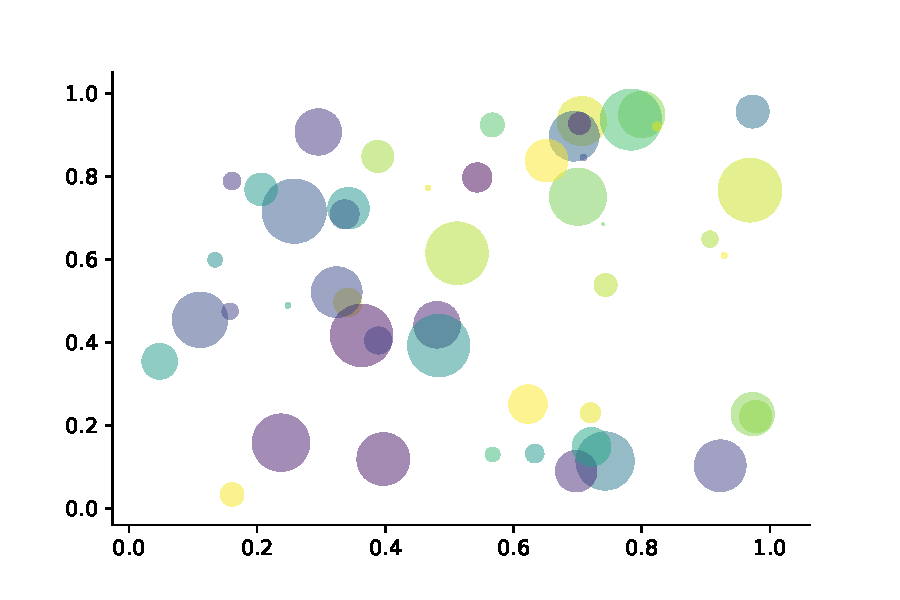
\includegraphics[width=0.6\textwidth]{scatter.pdf}
% 	\caption{Matplotlib: Scatter Plot Example\label{fig:mpg}}
% \end{figure}


% 回归分析(regression analysis) 是确定两种或两种以上变量间相互依赖的定量关系的一种统计分析方法。根据定理~ \ref{thm:fubi},其运用十分广泛,回归分析按照涉及的变量的多少,分为一元回归和多元回归分析;按照因变量的多少,可分为简单回归分析和多重回归分析;按照自变量和因变量之间的关系类型,可分为线性回归分析和非线性回归分析。

% 但是由于绝对值不易作解析运算,因此,进一步用残差平方和函数来度量总偏差。偏差的平方和最小可以保证每个偏差都不会很大。于是问题归结为确定拟合函数中的常数和使残差平方和函数最小。
% \begin{itemize}
% 	\item Routing and resource discovery;
% 	     \begin{itemize} 
%       	   	\item Language Models
%       	 	\item Vector Space Models
%     		 \end{itemize}
% 	\item Resilient and scalable computer networks;
% 	\item Distributed storage and search.
% \end{itemize}
% \section{示例}
% \begin{lstlisting}[frame=single]
% \documentclass[geye,green,pad,cn]{elegantnote}

% \title{Note Example}
% \author{ddswhu}
% \institute{Elegant\LaTeX{} Program}
% \version{1.00}
% \date{\today}

% \begin{document}

% \maketitle

% \section{Introduction}
% The content of Introduction.

% \end{document}
% \end{lstlisting}

\end{document}
